\chapter{Vorlesung 18}
\section{All-Pairs-Shortest Path Algorithmen}
Distanzmatrix $D$ für einen Graphen $G=(V,E)~~V={v_1,v_2,\ldots,v_n},~~w:E\mapsto\mathbb{R}$
\[ d_{ij}=\begin{cases}0&\text{für }i=j\\w(v_i,v_j)&\text{für }(v_i,v_j)\in E\\ \infty &\text{sonst}\end{cases} \]
\[D=(d_{ij})_{\substack{i=1,\ldots,n \\ j=1,\ldots, n}} \in \mathbb{R}^{n\times n}  \]
\begin{figure}[h]
\centering
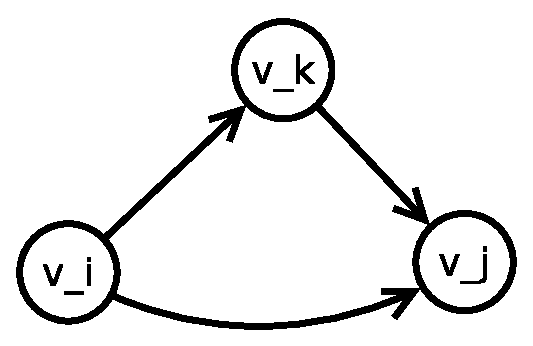
\includegraphics[width=0.2\linewidth]{18/Grafik/Diagramm1}
\caption{Grafik}
\label{fig:Diagramm1}
\end{figure}
\[ d^{(2)}_{ij} = \min(d^{(1)}_ij,~\underset{k=1,\ldots,n}{\min(d^{(1)}_{ik}+d^{(1)}_kj)}) \]
\[ D^{(2)} = D^{(1)}\circ D^{(1)}~~~~~=\min(d^{(1)}_{ik}+d^{(1)}_kj) \]
Vergleich zu Matrixmultiplikation
\[ C=A \circ B~~,\text{mit }A,B\in\mathbb{R}^{n\times n} \]
\[ C_{ij} = \sum_{k=1}^{n}a_{ik}\cdot b_{kj} \]
im Ring $(\mathbb{R},+,\cdot)$
\[ C_{ij} =  \underset{k=1,\ldots,n} (A_{ik}+B_{kj}) \]
\paragraph{Kommutativgesetz}
\[ \min(\min(a,b),c) = \min(a,b,c)\]
im "`Ring"'\footnote{der keiner ist} $(\mathbb{R}, \min, +)$
\paragraph{Distributivgesetz}
\[ a+\min(b,c) = \min(a+b, a+c) \]
\paragraph{Assoziativgesetz}
\[ A\circ (B \circ C) = (A \circ B) \circ C \]
\paragraph{Ziel:} $D^{(n)}\footnote{In der Potenz stehen die Anzahl der betrachteten Kanten. n entspricht allen Kanten} = D^{(1)}\circ D^{(1)}\circ \ldots\circ D^{(1)}$
\paragraph{Es gilt:} $D^{(n)} = D^{(n+m)}$ für $m\geq 1$
\subsection{Laufzeit zur Berechnung von $D^{(n)}$ }
\paragraph{Naiv:} $\mathcal{O}(n^4)$
\[ D^{(2)} = D^{(1)} \circ D^{(1)} \]
\[ D^{(4)} = D^{(2)} \circ D^{(2)} \]
\[ D^{(8)} = D^{(4)} \circ D^{(4)} \]
\[ \vdots\]
\[ D^{(2^i)} = D^{(2^{i-1})} \circ D^{(2^{i-1})} \]
Schrittzahl $i$ so wählen, dass $2^i \geq n$
\paragraph{sukzessives Quadrieren:} $\mathcal{O}(n^3\log n)$
\section{Floyd-Warshall-Algorithmus}
\begin{lstlisting}
for ( k = 1; k <= n; k++)
  for( i = 1; i <= n; i++)
    for ( j = 1; j <= n; j++)
      d[i][j] = min(d[i][j], d[i][k]+d[k][j])
\end{lstlisting}
\paragraph{Laufzeit} $\mathcal{O}(n^3)$
\subsection{Korrektheitsbeweis:}
\paragraph{Invariante} Nach dem k-ten Schleifendurchlauf entspricht $d_{ij}$ der Weglänge eines kürzesten Weges $p$ von $v_i$ nach $v_j$, 
wobei nur Zwischenknoten erlaubt sind, mit Index $\leq k$  \[p:v_i \rightarrow v_{l_1} \rightarrow v_{l_2} \rightarrow \ldots \rightarrow v_{l_m} \rightarrow v_j\]
d.h. $1\leq l_1,l_2,\ldots,l_m\leq k$
\pagebreak
\subsection{Beweis der Invariante durch Induktion nach $k$}
\begin{description}
\item[$k=0$:] Nach der Initialisierung von $D$, also vor dem 1. Schleifendurchlauf, gilt obige Invariante.
\item[$k-1\rightarrow k$:]$~$\\
\begin{figure}[H]
\centering
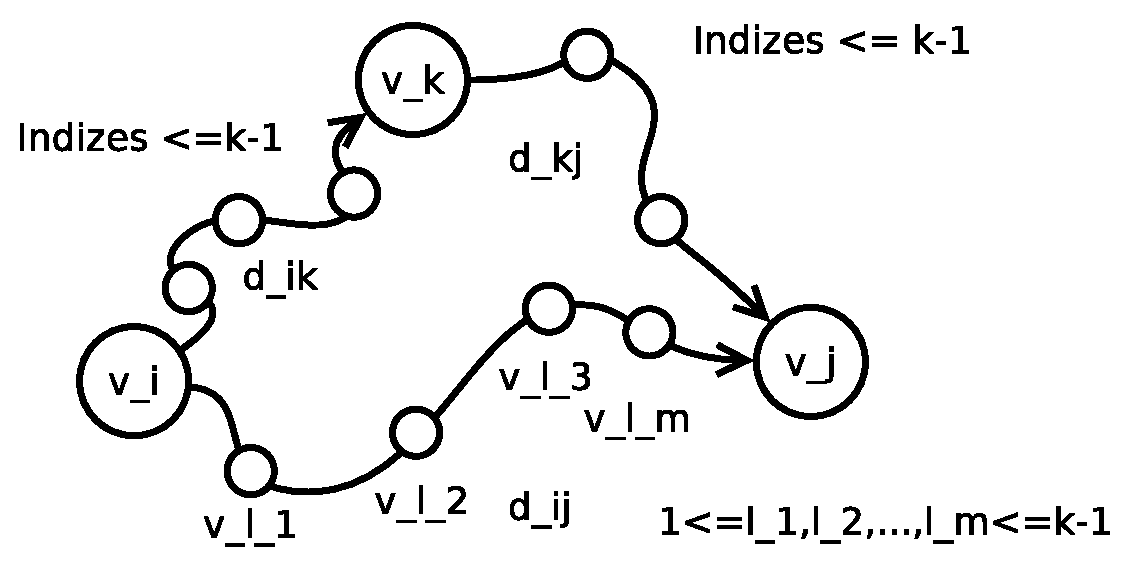
\includegraphics[width=0.5\linewidth]{18/Grafik/Diagramm2}
\caption{Beweis der invariante}
\label{fig:Diagramm2}
\end{figure}
Durch die Operation $d_{ij} = \min(d_{ij}, d_{ik}+d_{kj})$ wird die Invariante sichergestellt.
\end{description}
\section[Naive lösung]{Naive Lösung des All-Pairs Problems durch $|V|$-malige Anwendung von Bellman-Ford oder Dijksta-Algorithmus}
\begin{description}
\item[Bellman-Ford] $\mathcal{O}(|V|\cdot|V|\cdot|E|) = \mathcal{O}(|V|^2\cdot|E|)$
\item[Dijksra] $\mathcal{O}(|V|\cdot(|V|\cdot\log|V|+|E|)) = \mathcal{O}(|V|\cdot|E|+|V|^2\cdot\log|V|)$
\end{description}
\section{Johnson-Algorithmus}
\paragraph{Idee:} Neugewichtung der Kanten, so dass keine negativen Kantengewichte mehr vorhanden sind. Anschließend $|V|$-mal Dijkstra-Algorithmus ausführen.

\paragraph{Naiver Ansatz}$~~$\\

\begin{figure}[H]
\centering
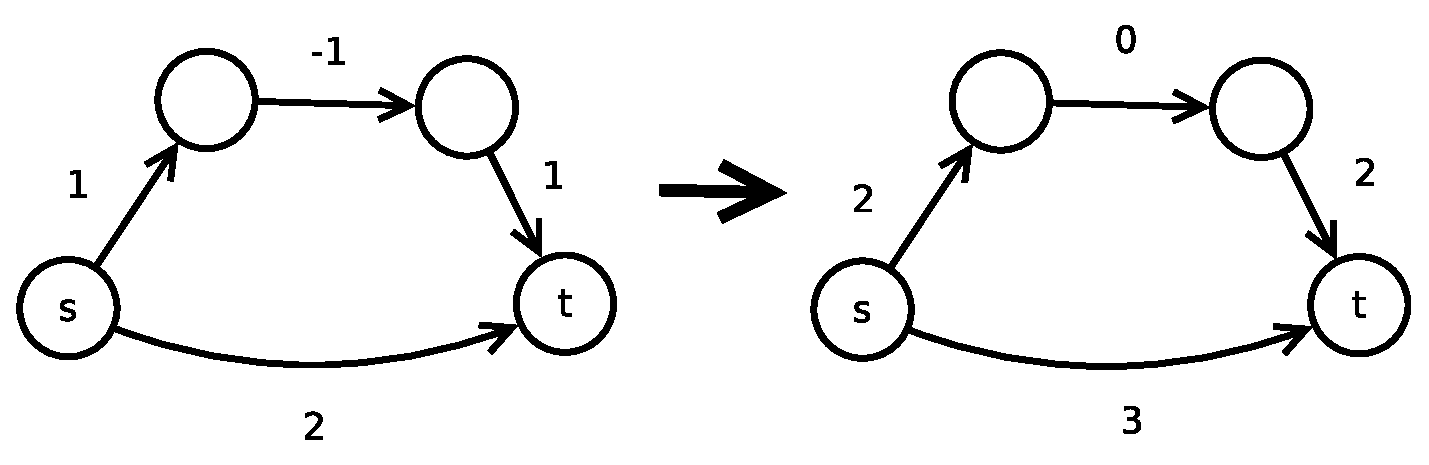
\includegraphics[width=0.7\linewidth]{18/Grafik/Diagramm3}
\caption{Naiver Ansatz, kürzester Weg wird zerstört}
\label{fig:Diagramm3}
\end{figure}
\pagebreak
\paragraph{Neuer Ansatz}
\[ w'(u,v) =\pot\footnote{Potentialfunktion}(u)-\pot(v)+w(u,v)\geq 0 \]
Mit dieser Neugewichtung gilt, dass kürzeste Wege bzgl. $w$ den kürzesten Wegen bzgl. $w'$ entsprechen.
\[ p:s=v_0\rightarrow v_1\rightarrow v_2\rightarrow \ldots v_i\rightarrow v_{i+1}\rightarrow\ldots v_k=t \]
\[ w'(p) = \sum_{i = 0}^{k-1} w'(v_i, v_{i+1}) = \sum_{i=0}^{k-1}\left[ \pot(v_i)-1\pot(v_{i+1}) +w(v_i, v_{i+1}) \right] \]
\[ \overset{Teleskopsumme}{=}\pot(v_0)-\pot(v_k)+\sum_{i = 1}^{k-1} w(v_i,v_{i+1}) = \pot(s)-\pot(t)+w(p) \]
\paragraph{d.h.}
Alle kürzesten Wege $s \rightsquigarrow t$ unterscheiden sich bzgl. $w'$ im Vergleich zu $w$ nur um eine feste additive Konstante $\pot(s)-\pot(t)$
\[ \pot(u)-\pot(v)+w(u,v) \geq 0 \]
\[ \pot(v)\leq \pot(u)+w(u,v)\footnote{Dreiecksungleichung} \]
%Grafik4
\[ \pot(v) = \delta(z,v) \]
\[ G'=(V',E')~~~ V'=V\cup{z}, E'=E\cup{(z,v) | v\in V} ~~~\text{mit }w'(z,v)=0\]
\begin{figure}[h]
\centering
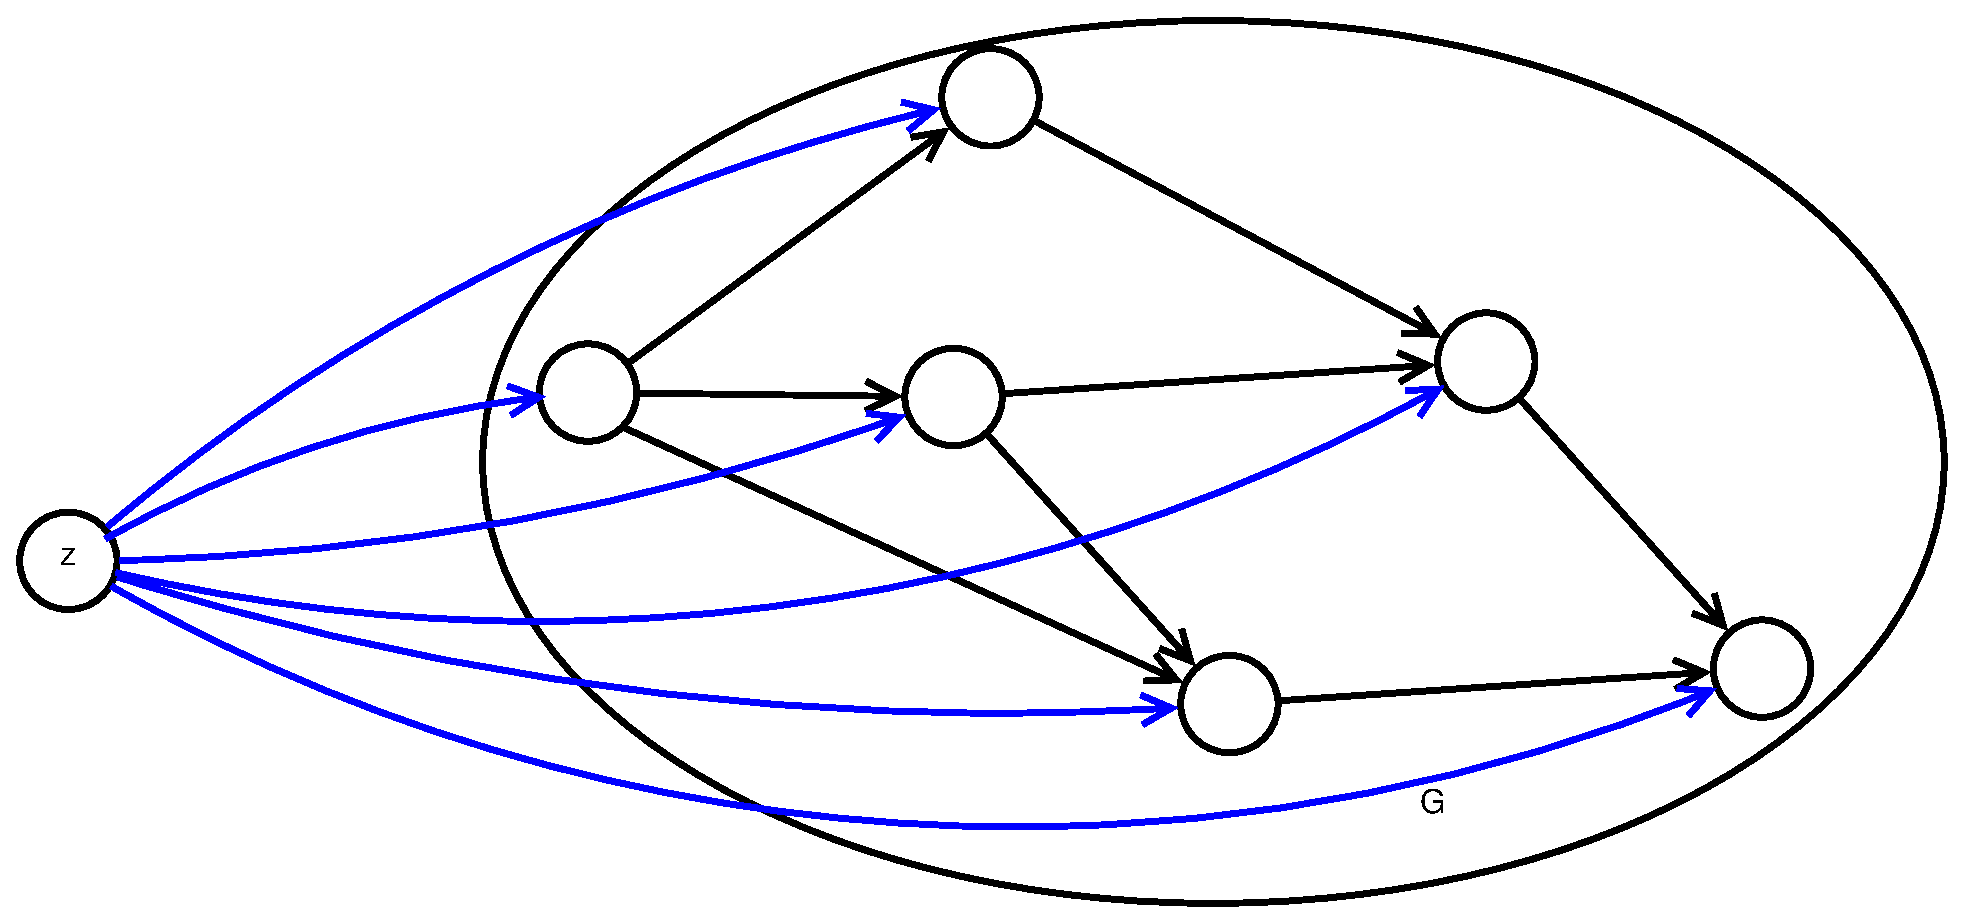
\includegraphics[width=0.7\linewidth]{18/Grafik/Diagramm5}
\caption{Die blau makierten Kanten haben die Länge 0}
\label{fig:Diagramm5}
\end{figure}

\begin{itemize}
	\item Löse single-source-shortest-Path Problem in $G'$ mit $z$ als Startknoten
	\item setze $\pot(v) = \delta_{G'}(z,v)\footnote{berechnet mit Bellman-Ford}$
	\item Neugewichtung
	\item $|V|$-mal Djikstra
\end{itemize}
\subsection{Laufzeit des Johnson-Algorithmus}
\[ \mathcal{O}(|V|\cdot|E|+|V|\cdot(|V|\cdot\log|V|+|E|)) = \mathcal{O}(|V|\cdot|E|+|V|^2\cdot|V|) \]